\documentclass{beamer}
\usepackage[utf8]{inputenc}
\usepackage[francais]{babel}
\usepackage[utf8]{inputenc}  
\usepackage{listings}
\usepackage{graphicx}
\usepackage{color}
\usepackage{float}
\usepackage{algorithm}
\usepackage{algorithmic}
\usepackage{caption}

\usepackage{array}
\usepackage{colortbl}
\usepackage{amsfonts}
\usepackage{geometry}
\usepackage{setspace}
\usepackage{hyperref}
\usepackage{subcaption}
\usepackage{listings}
\usetheme{Warsaw}
\setbeamertemplate{footline}[frame number]

\PassOptionsToPackage{demo}{graphicx}




\author{Adrien Guilbaud}
\title{Simulation numérique directe de la combustion turbulente}
%\subtitle{Presentation Subtile}
%\institute{Université de Bordeaux}
%\date{\today}


%\titlegraphic{
\includegraphics[width=2cm]{figures/logo_fac.jpg}\hspace*{4.75cm}~%
%   
\includegraphics[width=2cm]{figures/logo_cerfacs.eps}
%}

\def\mathunderline#1#2{\color{#1}\underline{{#2}}\color{black}}

\begin{document}
 \AtBeginSection[]
{
  \begin{frame}
    \frametitle{Table of Contents}
    \tableofcontents[currentsection]
  \end{frame}
}

\begin{frame}[plain]
    \parbox[c]{-50cm}{\centering%
      
\includegraphics[width=2cm]{figures/logo_fac.jpg}%
    }%
    \parbox[c]{19.5cm}{\centering%
      
\includegraphics[width=2cm]{figures/logo_cerfacs.eps}
    }%
\maketitle

\centering
\footnotesize
\begin{tabular}{cc}
  Maître de stage & Enseignant responsable \\
  Mme.~Isabelle \textsc{D'ast} &   Mr.~Samuel \textsc{Thibault} \\
  \end{tabular}
\end{frame}

%
% INTRO
%

\section{Introduction}
\subsection{Présentation du Cerfacs}
\begin{frame}
  \begin{itemize}
  \item Centre de recherche en calcul scientifique
  \item Actionnaires: Airbus Group, Cnes, EDF, Météo France, Onera, Safran et Total
  
    \item Résolution de problèmes scientifiques par la résolution numérique liés :
	\begin{itemize}
  \item au climat
  \item à l'aéronautique
  \item au spatial
  \item à l'environnement
  \end{itemize}
  \end{itemize}


  
\end{frame}

%https://en.wikipedia.org/wiki/Discretization_of_Navier%E2%80%93Stokes_equations
\subsection{Mécanique des fluides numérique}
\begin{frame}
  \begin{block}{Mécanique des fluides}
    Etude du comportement des fluides lorsqu'ils sont en mouvement
  \end{block}
  
  \begin{itemize}
  \item Résolution des équations de Navier-Stokes (équations aux dérivées partielles)
  \item Mécanique des fluides numérique $\implies$ discrétisation de l'espace
  \end{itemize}
\end{frame}


\subsection{Simulation de la turbulence}
\begin{frame}
  Écoulement turbulent $\implies$ apparition de tourbillons instables
  \begin{itemize}
  \item \textit{DNS}: Direct Numerical Simulation
  \item \textit{LES}: Large Eddy Simulation
  \end{itemize}

  \begin{figure}[ht]
  \centering
  \begin{subfigure}[b]{0.5\textwidth}
    \centering
    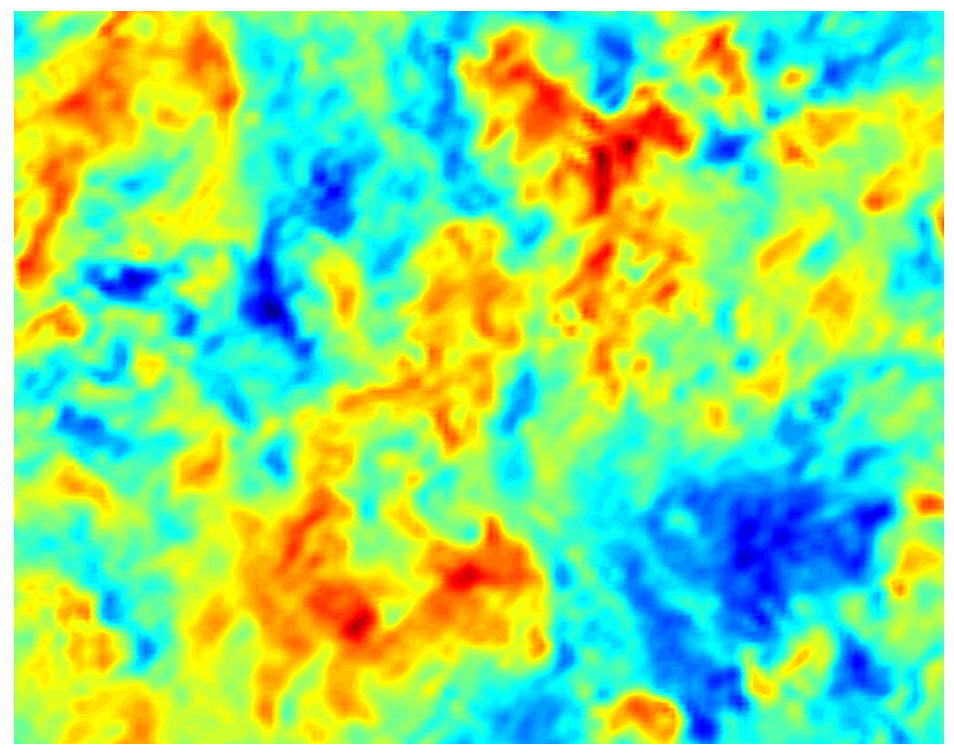
\includegraphics[scale=0.25]{figures/DNS_Velocity_Field.png}
    \caption{\label{fig:dns} DNS}
  \end{subfigure}%
  ~
  \begin{subfigure}[b]{0.5\textwidth}
    \centering
    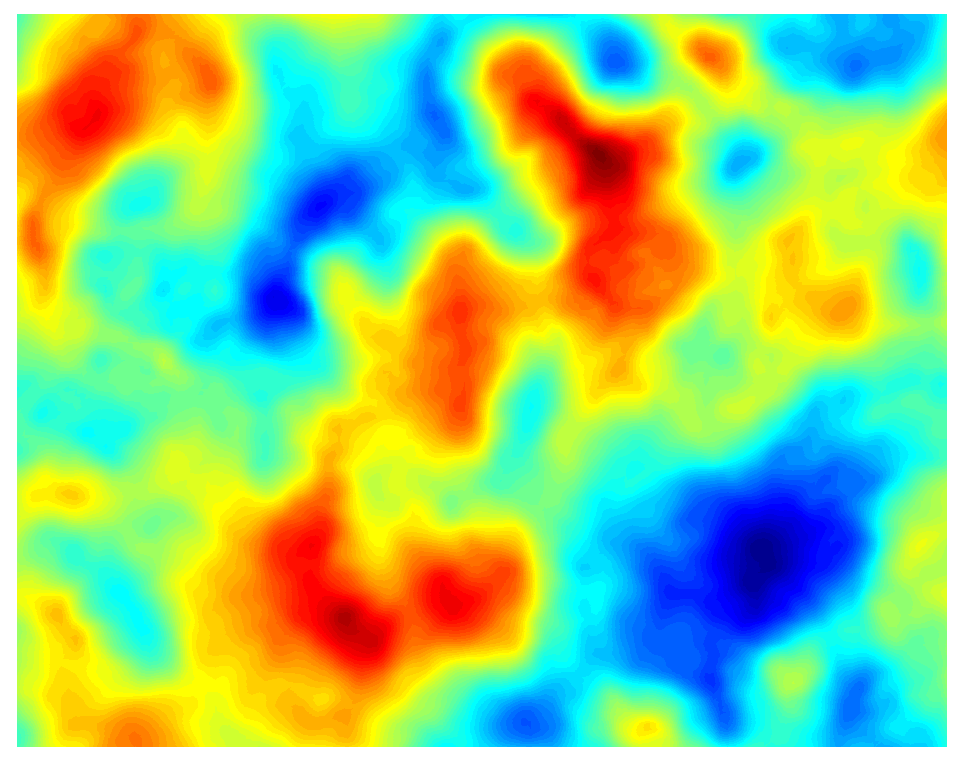
\includegraphics[scale=0.25]{figures/DNS_Filtered_Velocity_Field_Large.png}
    \caption{\label{fig:les} LES}
  \end{subfigure}
\end{figure}
\end{frame}




%
% Présentation stage
%
\section{Présentation du stage}
\subsection{NTMIX\_CHEMKIN}
\begin{frame}
  \textit{NTMIX\_CHEMKIN}: solveur d'écoulements réactifs
  \begin{itemize}
  \item bidimensionnel
  \item approche DNS
  \item couplé avec \textit{CHEMKIN}
  \end{itemize}
  
  \vfill
  Intérêt en recherche fondamentale
  
\end{frame}


\subsection{Objectifs}
\begin{frame}

  \begin{block}{Objectif}
    Développer une version 3D et parallèle de \textit{NTMIX}
  \end{block}
  \begin{itemize}
  \item Modernisation du code
  \item Développement de la version tridimensionnelle
  \item Parallélisation la version 3D
  \item Étude des performances
  \end{itemize} 
\end{frame}


%
% Parallélisation
%

\section{Parallélisation de NTMIX}
\subsection{Décomposition de domaine}
\begin{frame}
  \begin{block}{Objectif}
    Exécuter NTMIX sur de grands maillages ($\approx 10^9$ points)
  \end{block}
  \pause
  \begin{alertblock}{Limitations matérielles}
    \begin{itemize}
    \item     Mémoire minimum nécessaire: $10^9pts \times 5 \times 8o \approx 37.25$ Go
    \item     Temps de calcul: $10^9 pts\times(4\times10^{-6})s/p\times10000it\approx463jours$
    \end{itemize}
  \end{alertblock}
  
\end{frame}


\begin{frame}

    \centering
    \only<1>{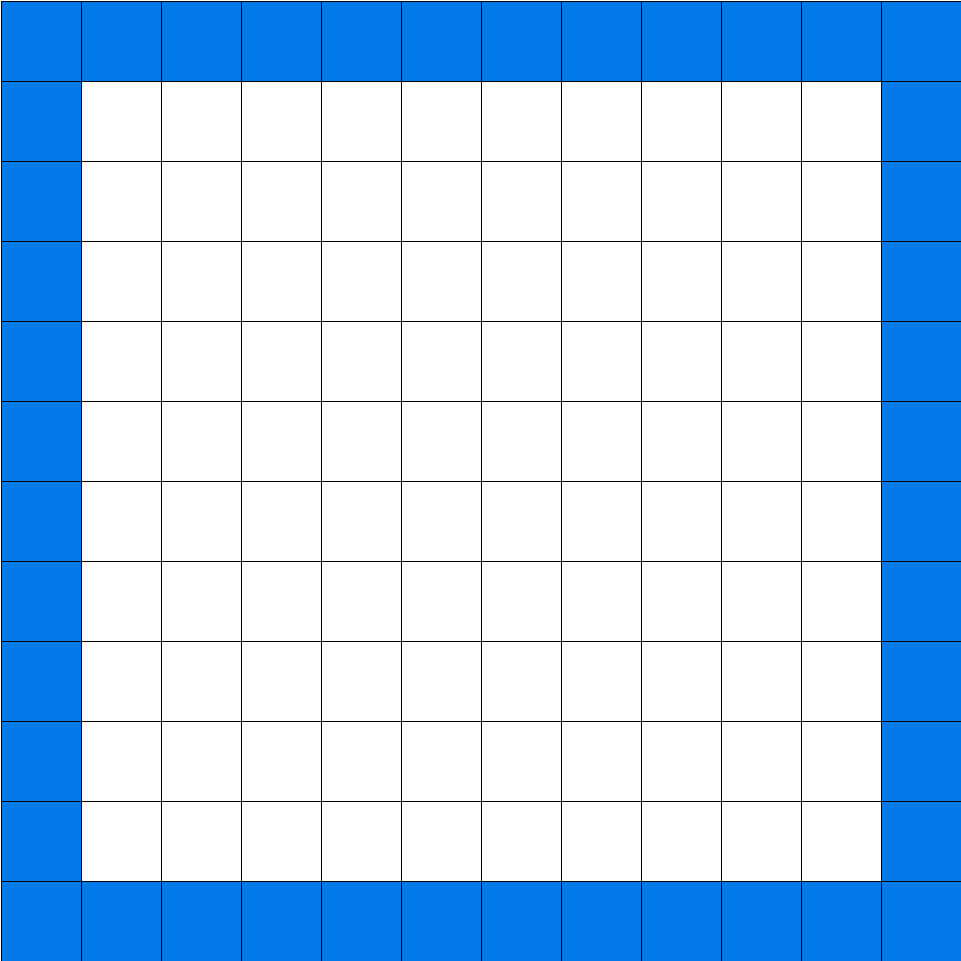
\includegraphics[scale=0.15]{figures/globaldomain.png}\\}
    \only<2>{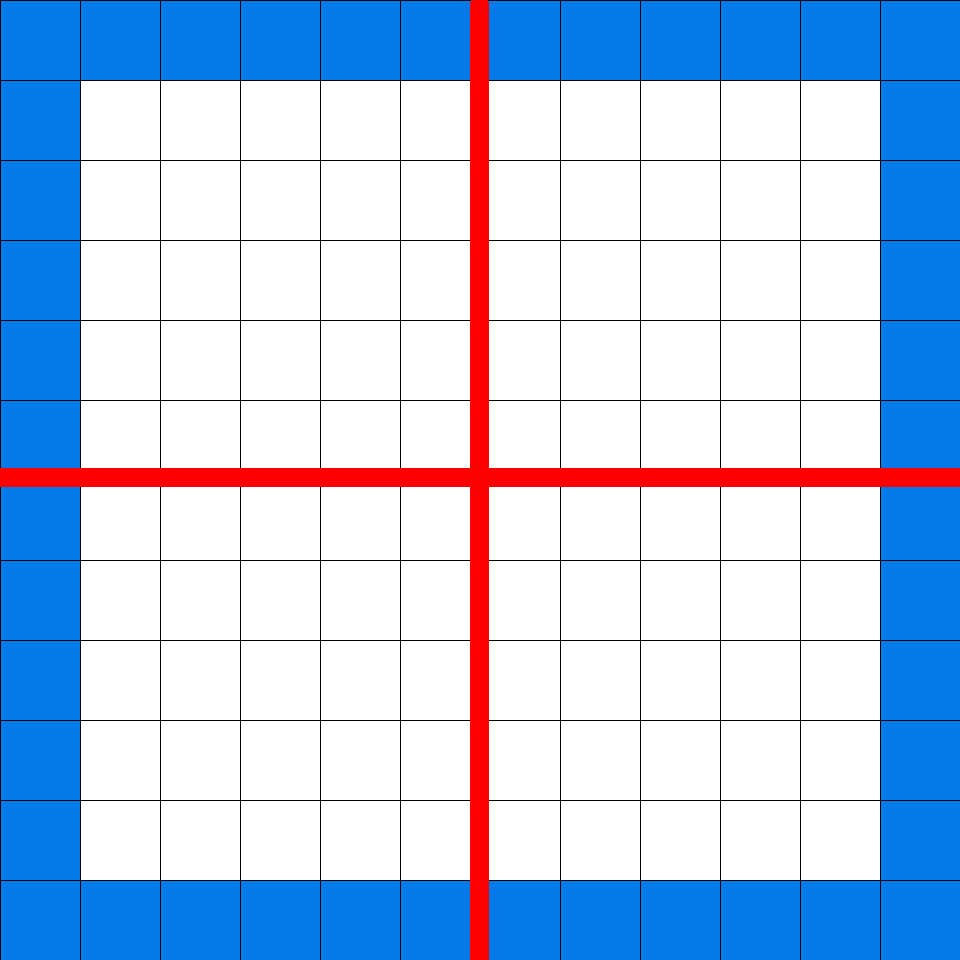
\includegraphics[scale=0.15]{slide_domain_cut.png}\\}
\end{frame}




\begin{frame}
  \begin{alertblock}{Problème}
    Les points des bordures internes manque d'informations
  \end{alertblock}

\footnotesize

\only<2>{$$3\left( \frac{\partial u}{\partial x}\right) _{i-1} + 9\mathunderline{green}{\left( \frac{\partial u}{\partial x}\right) _{i}} + 3\left( \frac{\partial u}{\partial x}\right) _{i+1} = \frac{1}{h}\left(  \frac{1}{4} \left( u_{i+2}-u_{i-2} \right) + 7 \left( u_{i+1} - u_{i-1} \right) \right) $$}


\only<3>{$$3\left( \frac{\partial u}{\partial x}\right) _{i-1} + 9\mathunderline{green}{\left( \frac{\partial u}{\partial x}\right) _{i}} + 3\left( \frac{\partial u}{\partial x}\right) _{i+1} = \frac{1}{h}\left(  \frac{1}{4} \left( \mathunderline{red}{ u_{i+2}}-\mathunderline{red}{u_{i-2}} \right) + 7 \left( \mathunderline{red}{u_{i+1}} - \mathunderline{red}{u_{i-1}} \right) \right) $$}

\only<4>{$$3\mathunderline{red}{\left( \frac{\partial u}{\partial x}\right) _{i-1}} + 9\mathunderline{green}{\left( \frac{\partial u}{\partial x}\right) _{i}} + 3\mathunderline{red}{\left( \frac{\partial u}{\partial x}\right) _{i+1}} = \frac{1}{h}\left(  \frac{1}{4} \left( \mathunderline{red}{ u_{i+2}}-\mathunderline{red}{u_{i-2}} \right) + 7 \left( \mathunderline{red}{u_{i+1}} - \mathunderline{red}{u_{i-1}} \right) \right) $$}

\end{frame}

\begin{frame}
  \centering
    \only<1>{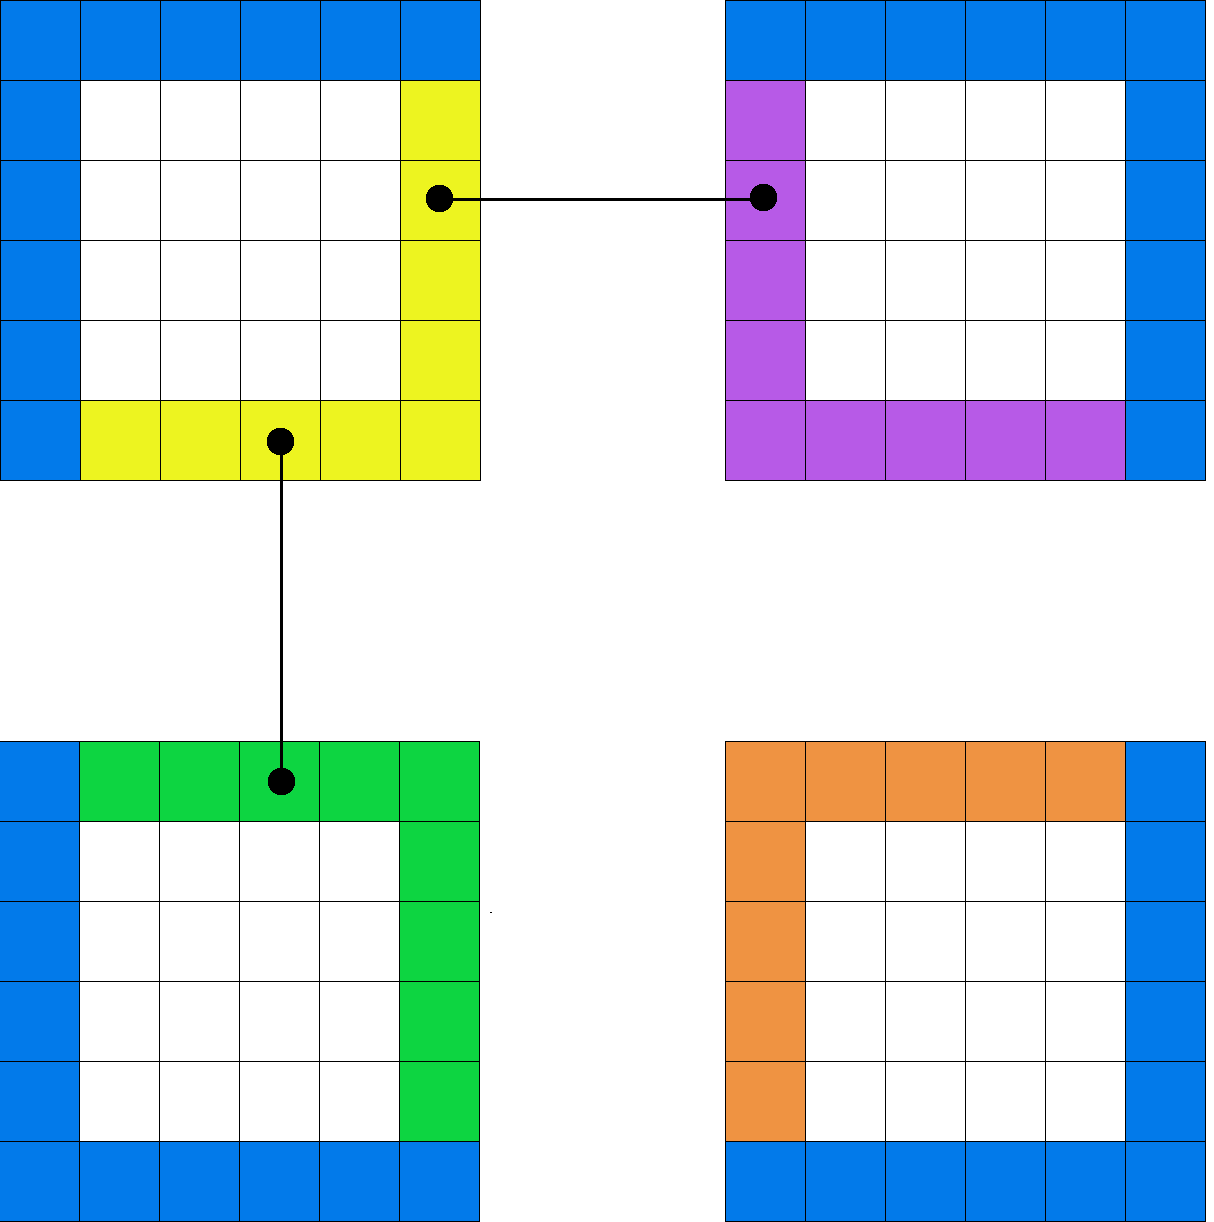
\includegraphics[scale=0.15]{figures/depdomain.png}\\}
    \only<2>{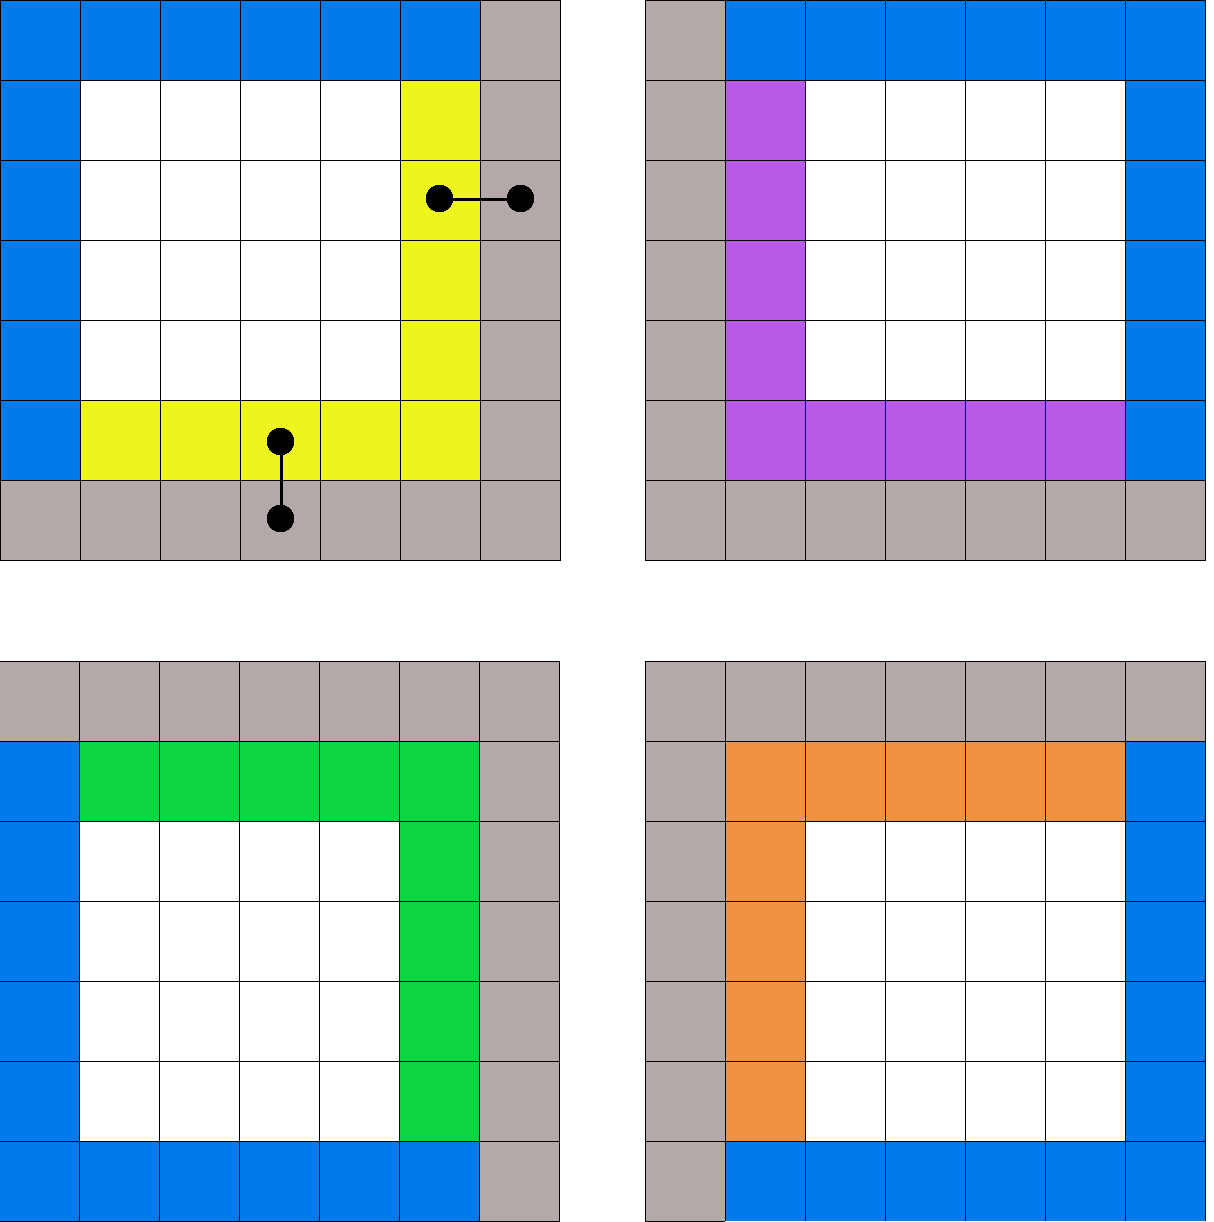
\includegraphics[scale=0.15]{figures/depdomain-overlap.png}}
  
\end{frame}


\begin{frame}
  \begin{itemize}
  \item   Traitement des bordures du domaine ?
  \item   Utilisation d'un schéma décentré
  \end{itemize}

 
  \footnotesize
    \begin{subequations}
    \begin{align*}
    \left( \frac{\partial u}{\partial x}\right) _{i-1} + 4 \left( \frac{\partial u}{\partial x}\right) _{i}  +  \left( \frac{\partial u}{\partial x}\right) _{i-1} &= \frac{1}{h}\left( \frac{1}{3} \left( u_{i+1} - u_{i-1} \right) \right)
    \end{align*}
  \end{subequations}
  
\end{frame}


%\begin{frame}
%  Méthode Schwarz:
%  \begin{itemize}
%  \item Couplage inter-domaine élevé
%  \item $\nearrow$ communications
%  \item $\searrow$ taille des communications
%  \end{itemize}
%  Problème local modifié:
%  \begin{itemize}
%  \item Couplage inter-domaine faible
%  \item $\searrow$ communications
%  \item $\nearrow$ taille des communications
%  \end{itemize}
%\end{frame}


%\begin{frame}
%
%  \centering
%    \only<1>{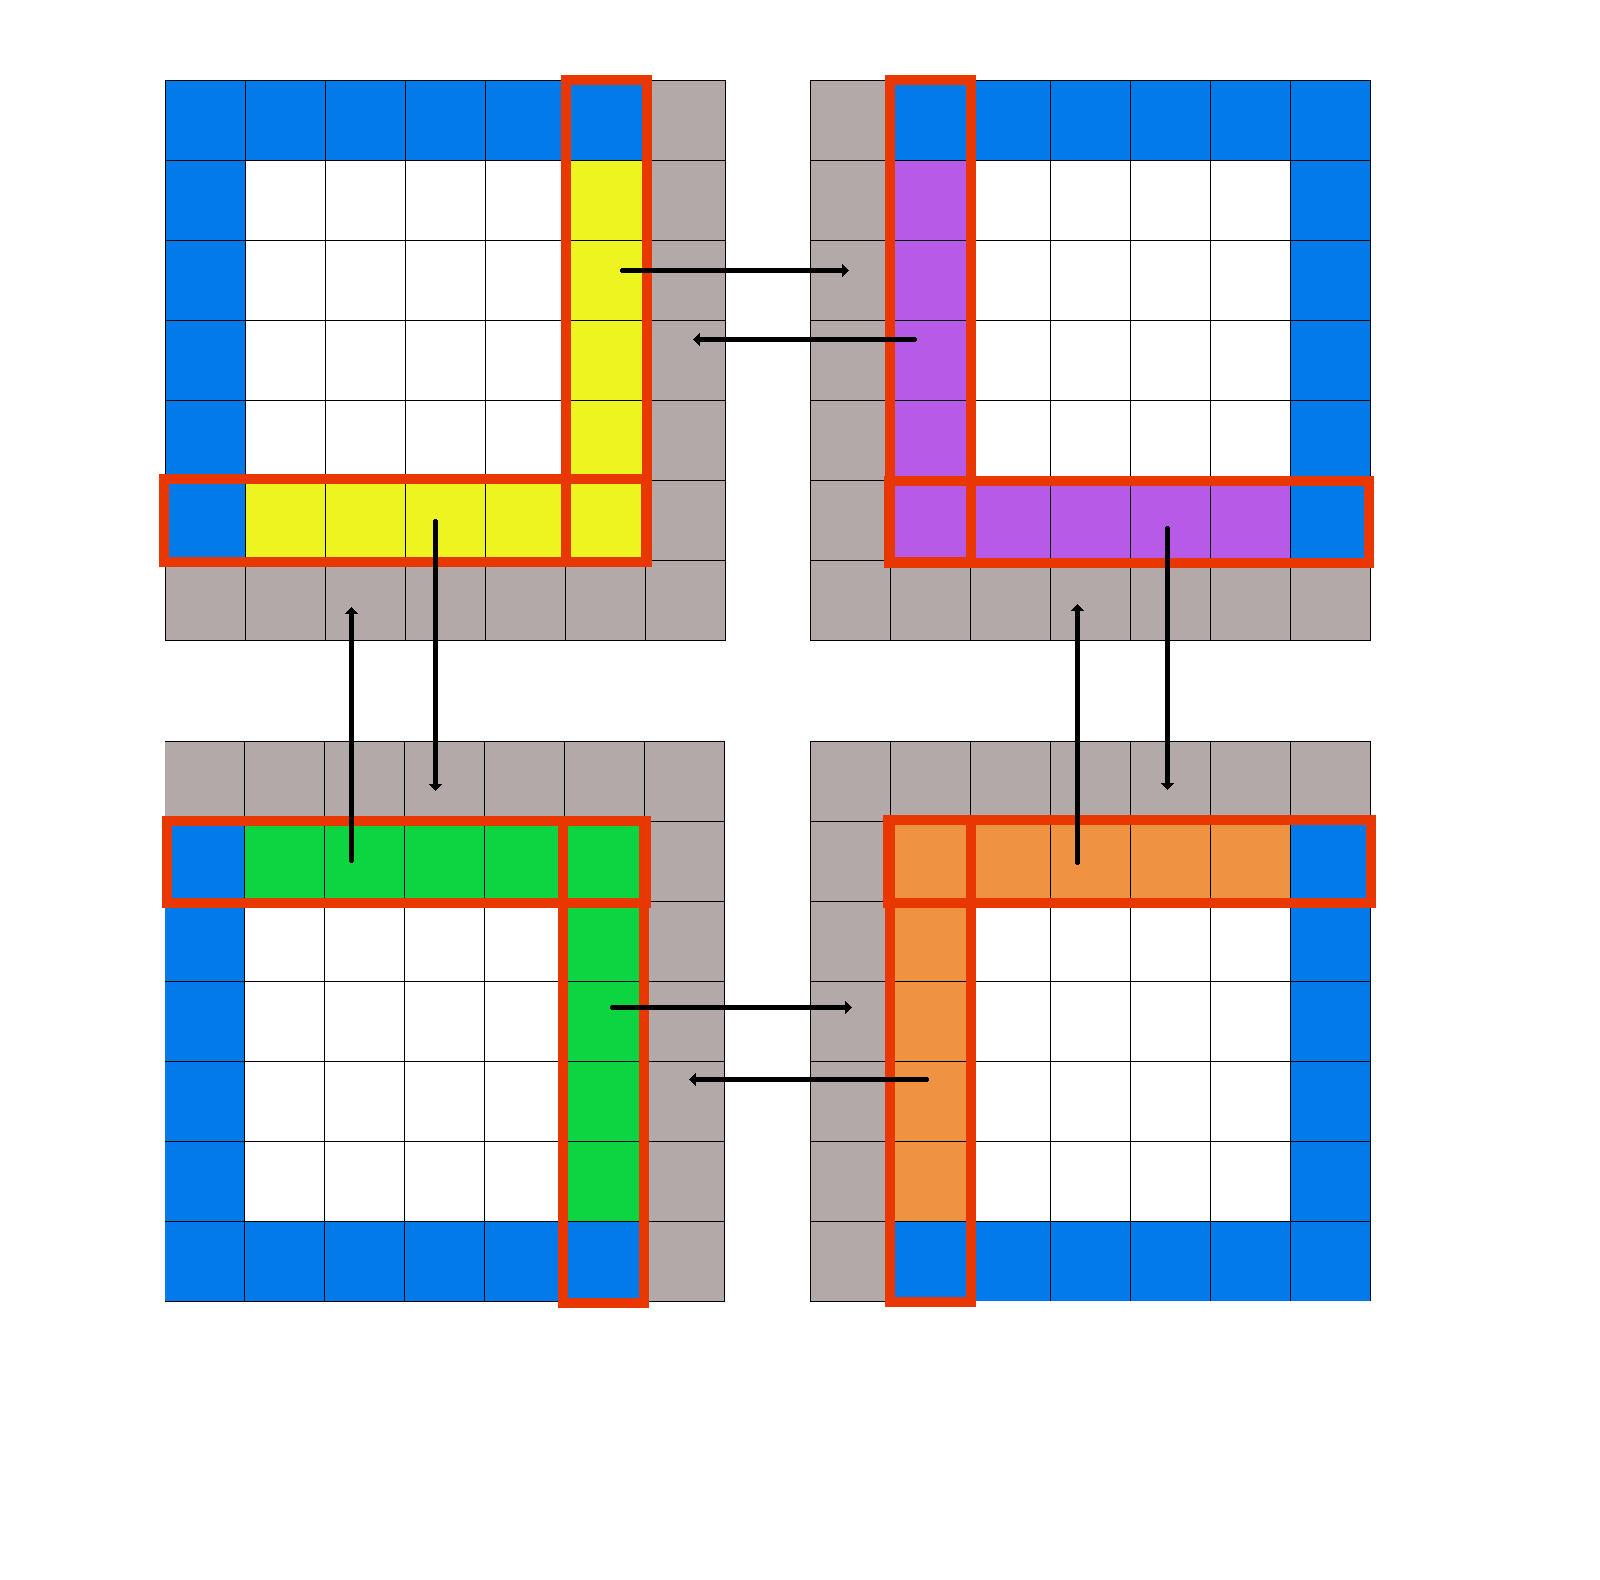
\includegraphics[scale=0.15]{slide_neigh_1.png}\\}
%    \only<2>{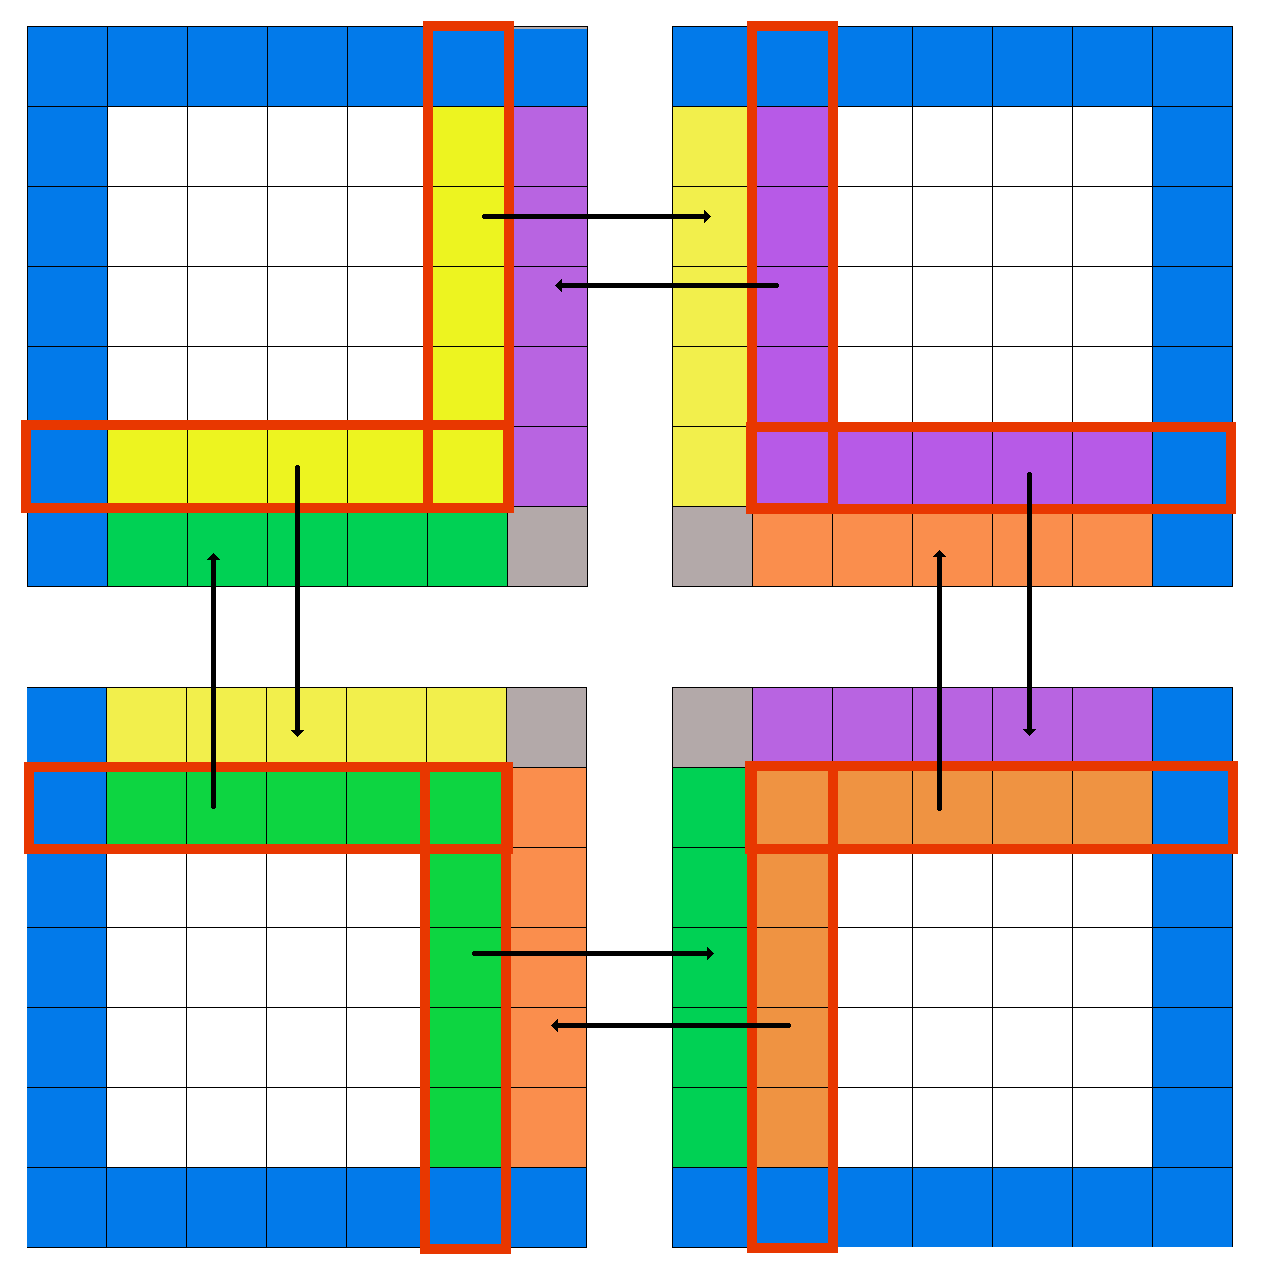
\includegraphics[scale=0.15]{slide_neigh_2.png}\\}
%    \only<3>{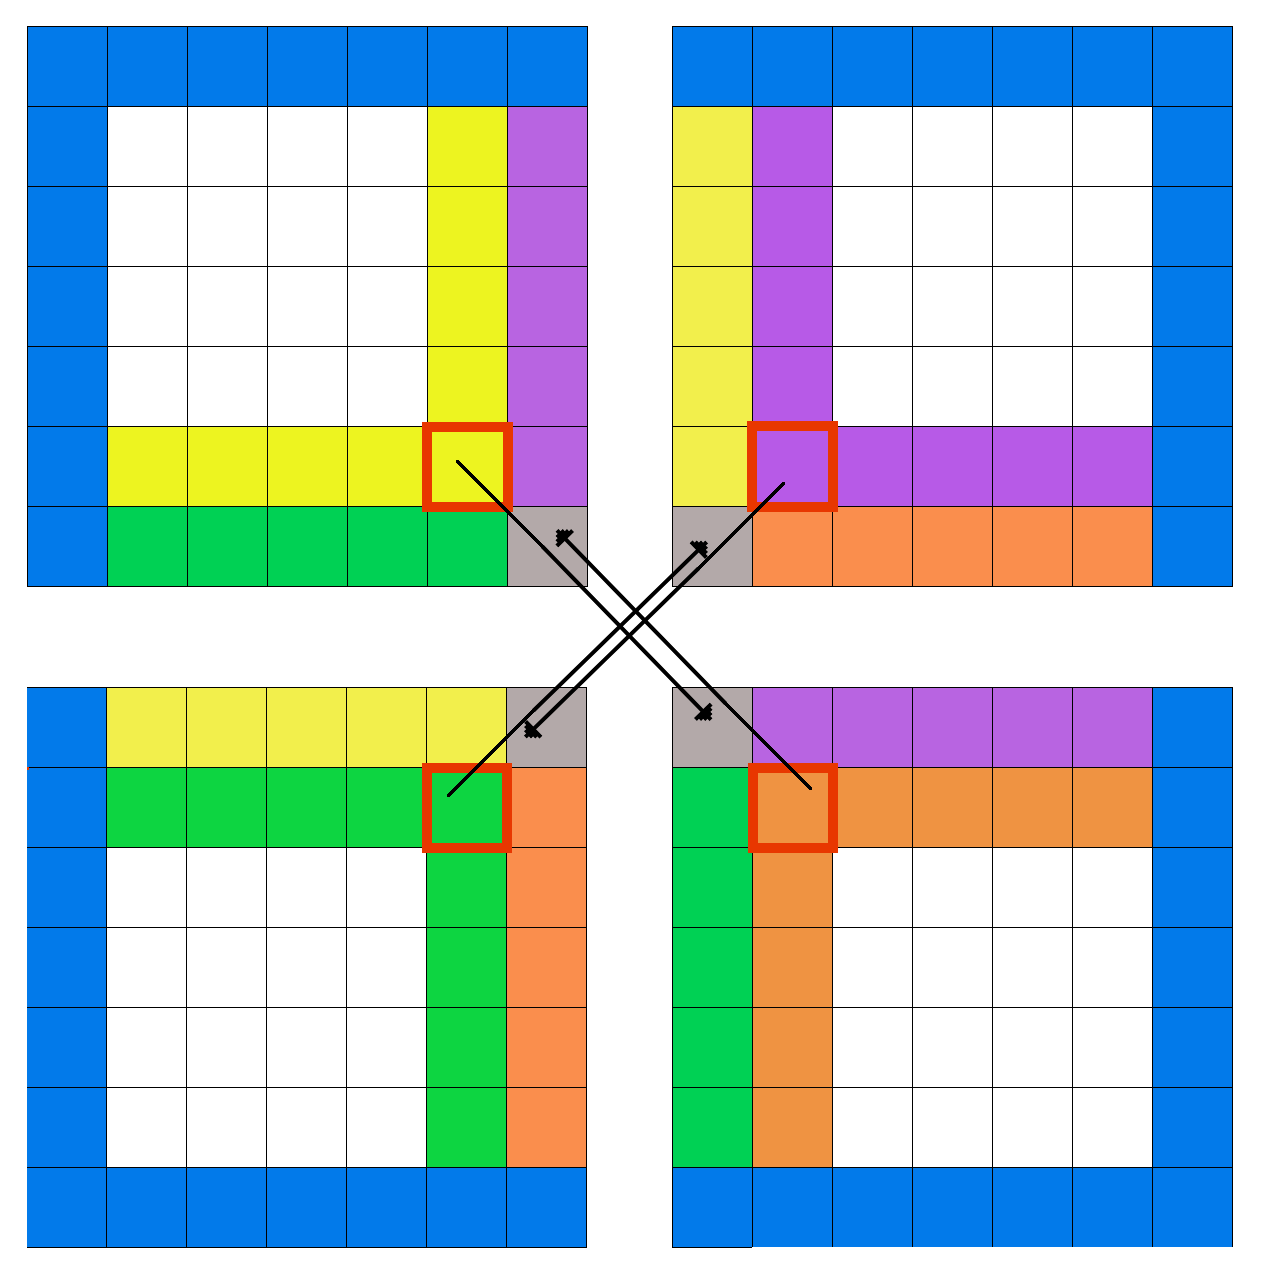
\includegraphics[scale=0.15]{slide_neigh_3.png}\\}
%    \only<4>{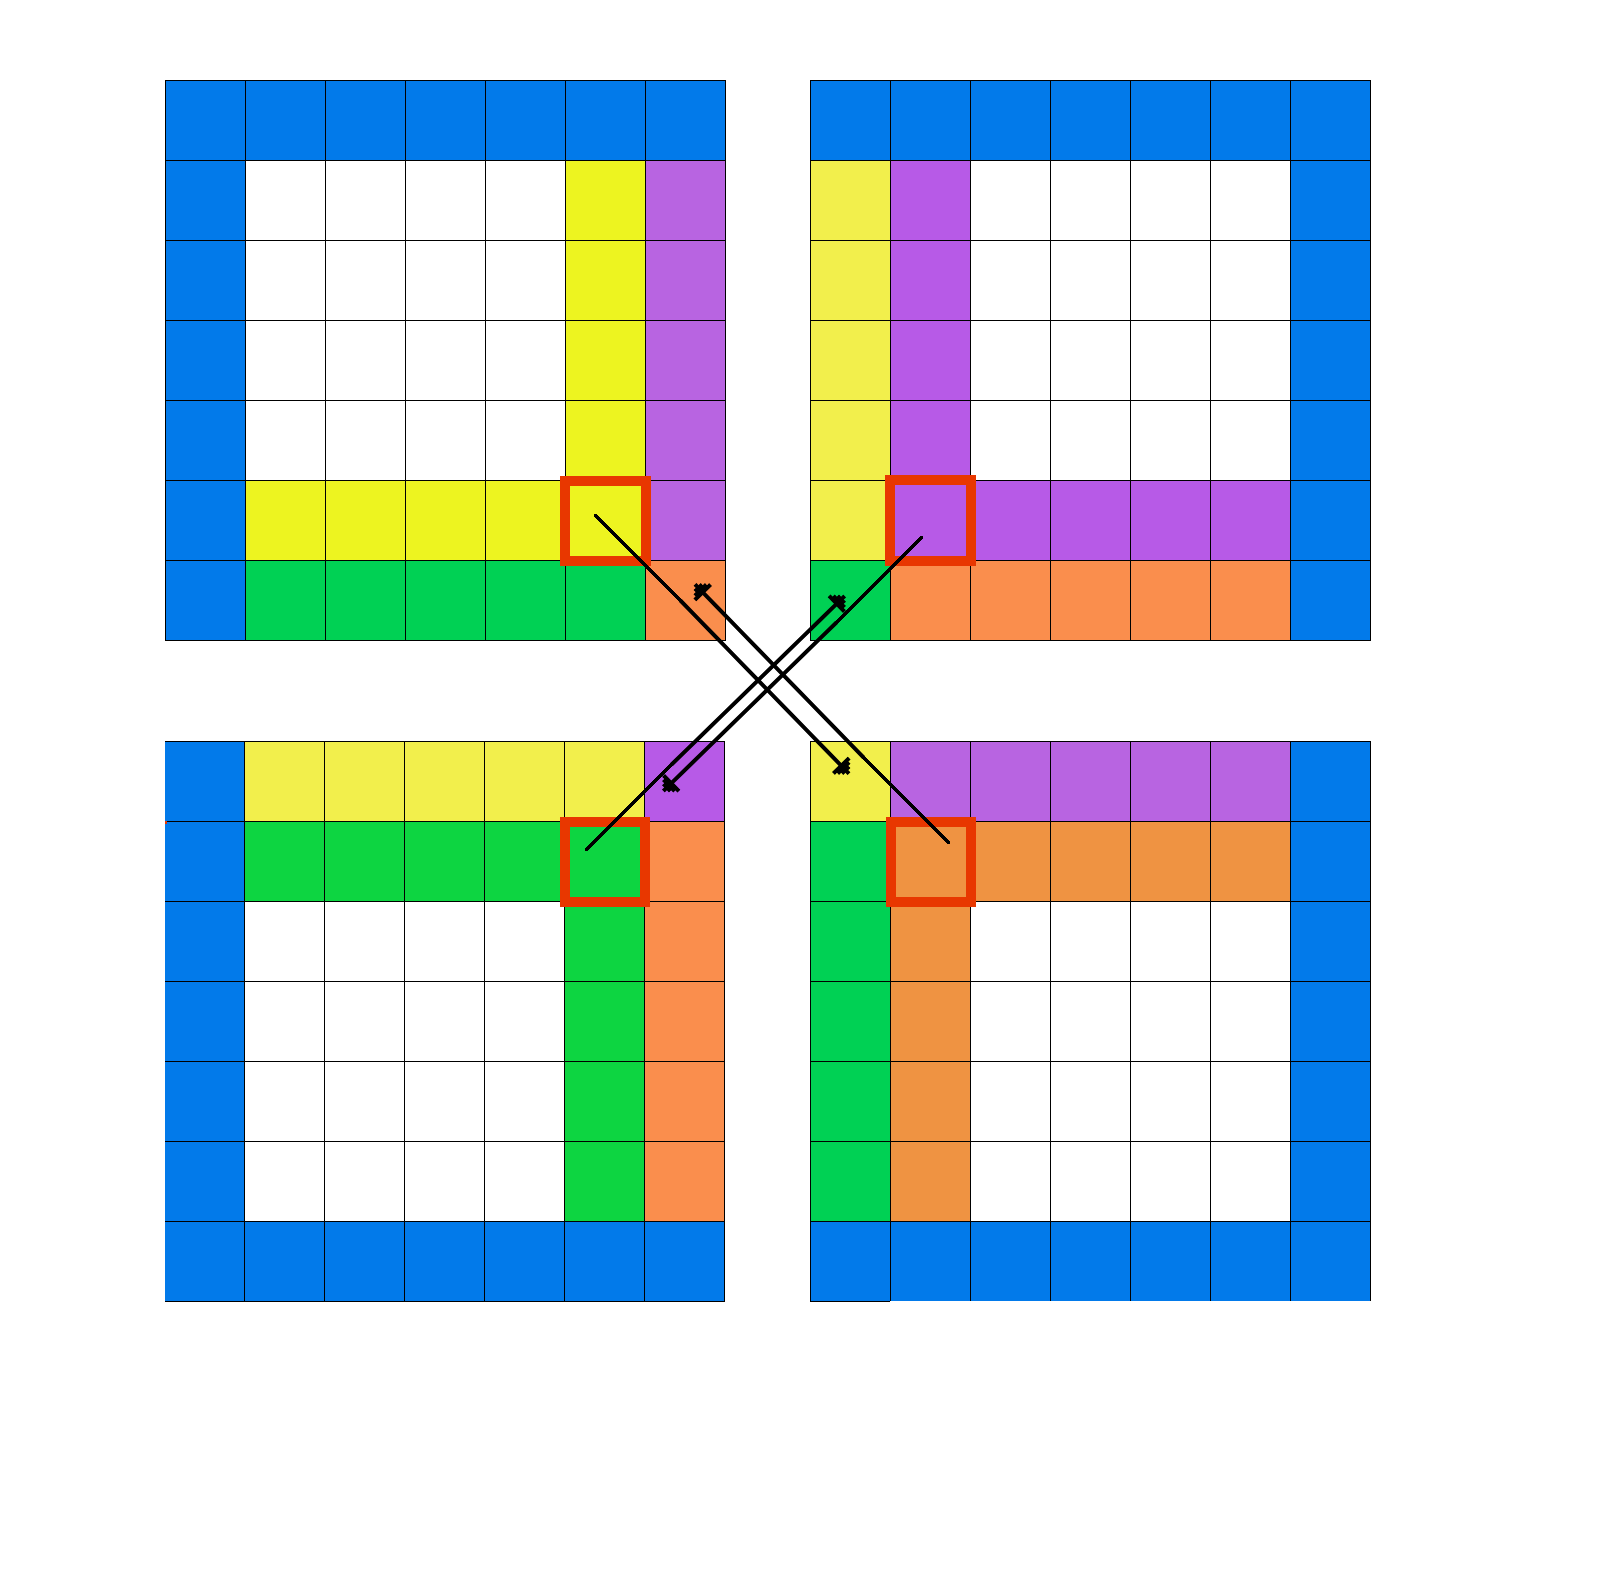
\includegraphics[scale=0.15]{slide_neigh_4.png}}
%\end{frame}

\subsection{Communications}
\begin{frame}
  \begin{itemize}
  \item Discrétisation temporelle (méthode de Runge-Kutta)
  \item 1 communication des points de recouvrement/itération
  \item Duplication de calculs
  \end{itemize}

\only<2->{  \begin{algorithm}[H]
    \algsetup{linenosize=\small}
    \scriptsize
    \caption{time\_step}
    \label{algo:time_step}
    \begin{algorithmic}
      \only<3>{\STATE {Call Update}}
      \only<2->{\STATE {Call RHS(1)}}
      \only<3>{\STATE {Call Update}}
      \only<2->{\STATE {Call RHS(2)}}
      \only<3>{\STATE {Call Update}}
      \only<2->{\STATE {Call RHS(3)}}
    \end{algorithmic}
  \end{algorithm}}
  
\end{frame}

\begin{frame}
  Échanges des points de recouvrement
  \centering
    \only<1>{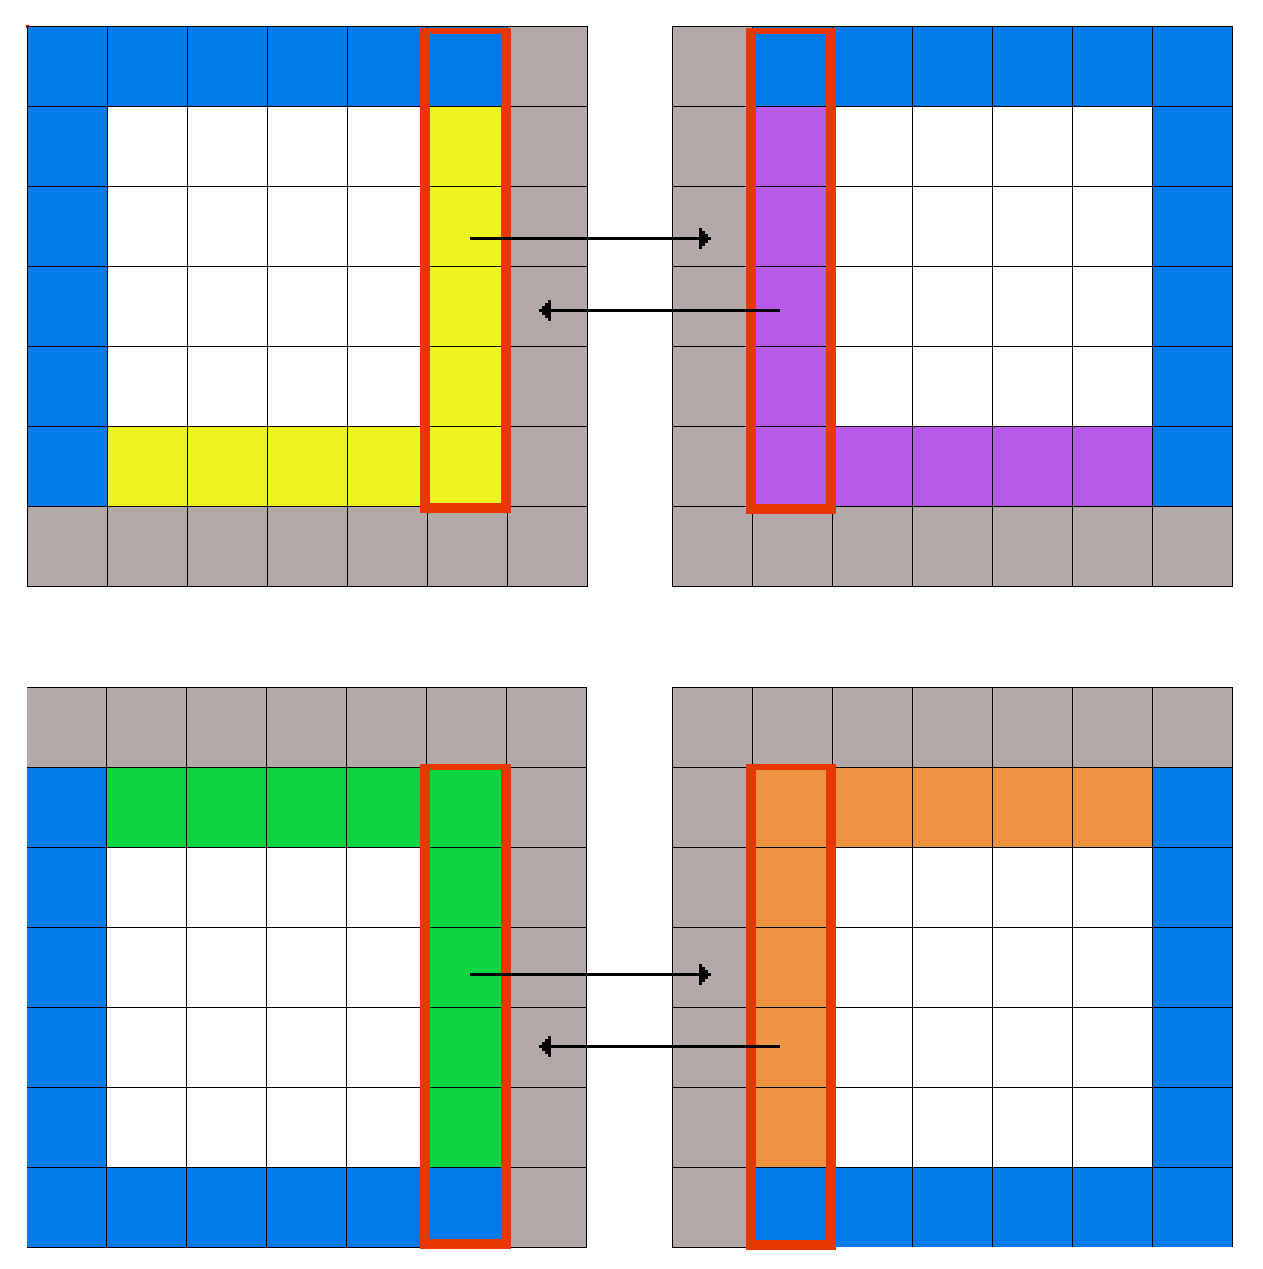
\includegraphics[scale=0.15]{slide_cust_1.png}\\}
    \only<2>{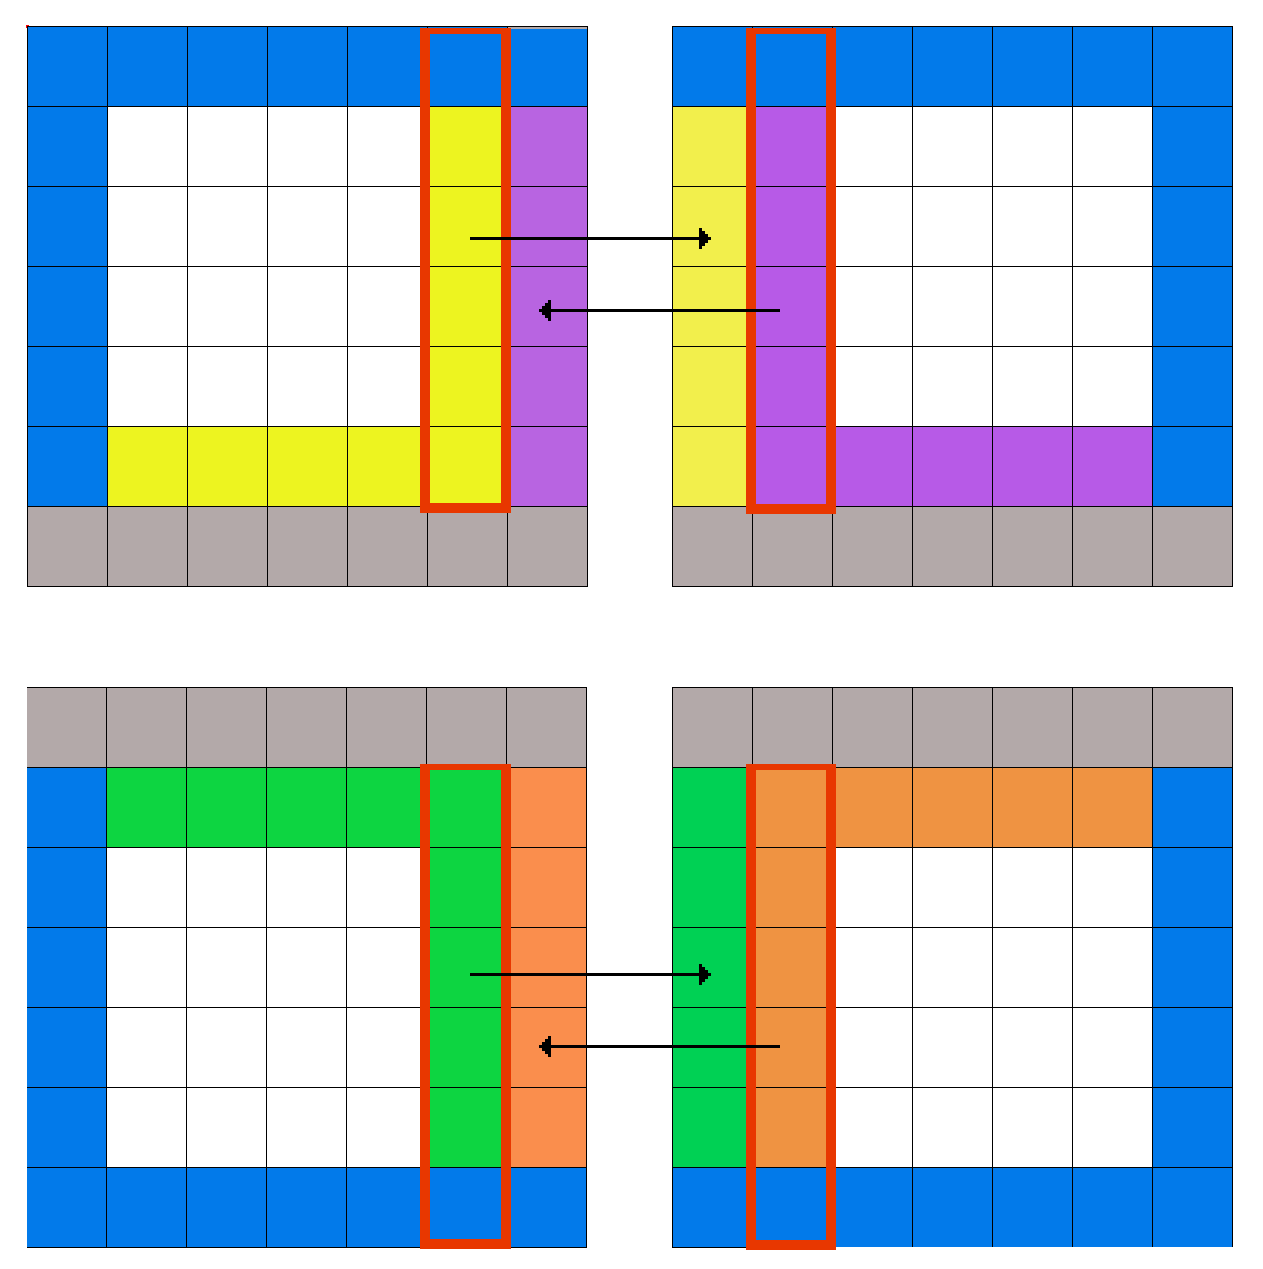
\includegraphics[scale=0.15]{slide_cust_2.png}\\}
    \only<3>{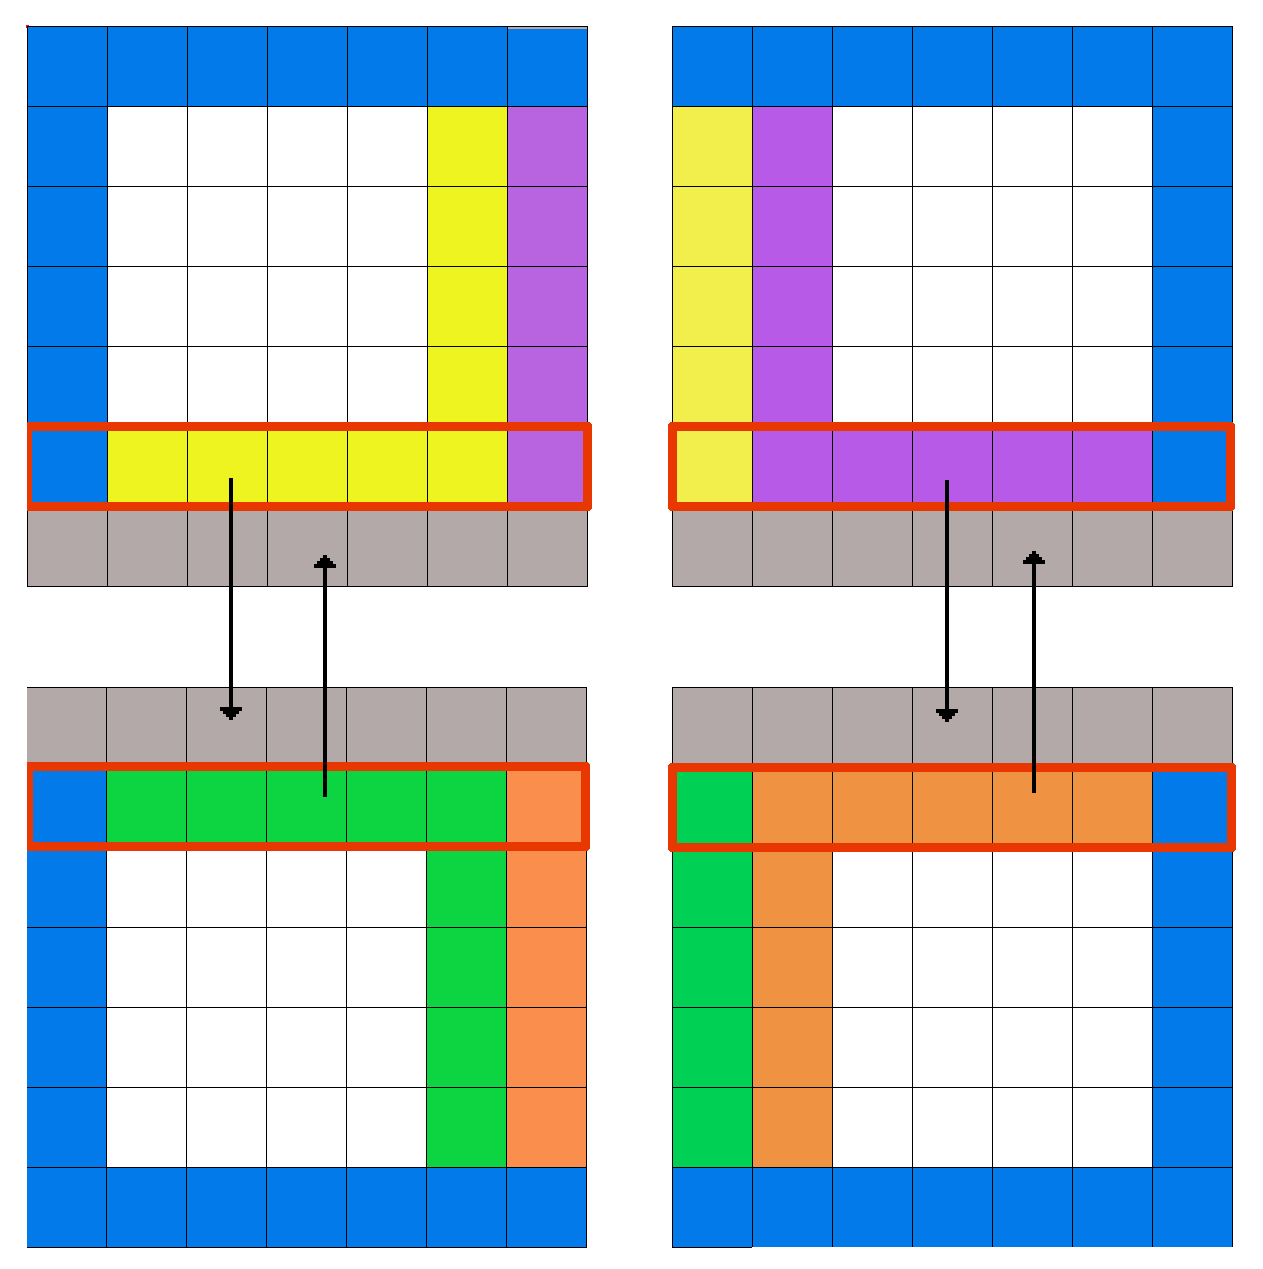
\includegraphics[scale=0.15]{slide_cust_3.png}\\}
    \only<4>{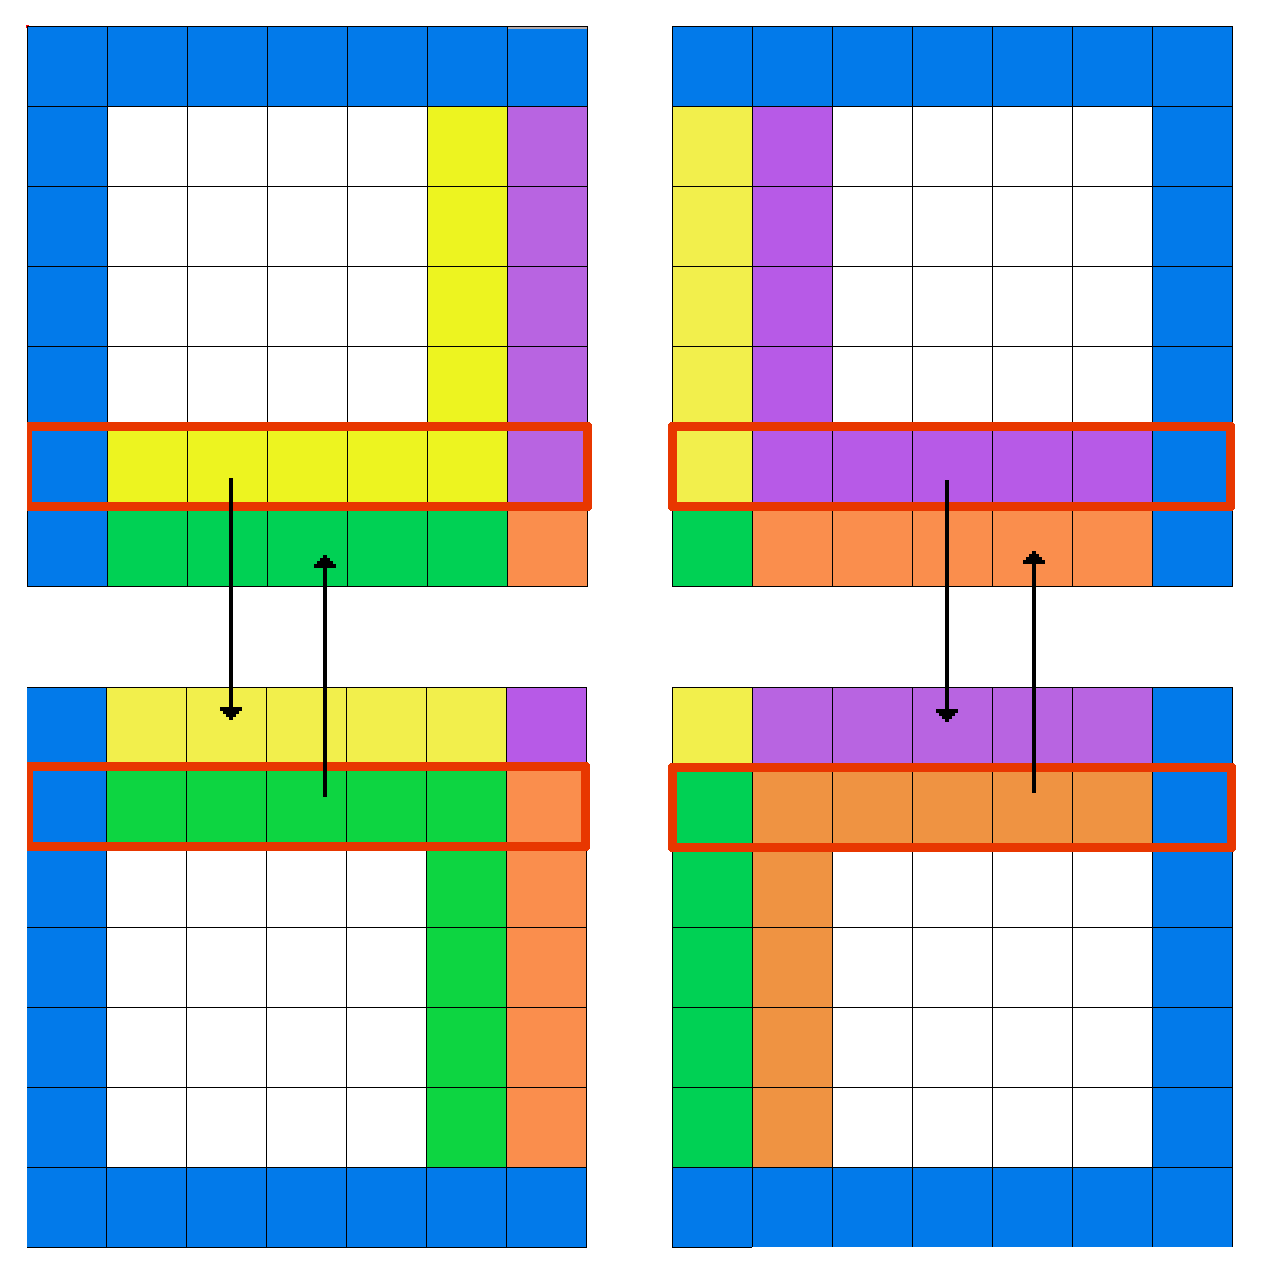
\includegraphics[scale=0.15]{slide_cust_4.png}}
\end{frame}


%
% Performances
%

\section{Etude des performances}
\subsection{Scalabilité forte}
\begin{frame}
  Scalabilité forte:
  \begin{itemize}
  \item domaine global de $400^3$
  \item augmentation progressive du nombre de noeuds
  \end{itemize}
  \vfill
  Efficacité: $$E=\frac{t_1}{n\times t_n}$$
\end{frame}


\begin{frame}
  \centering
    \only<1>{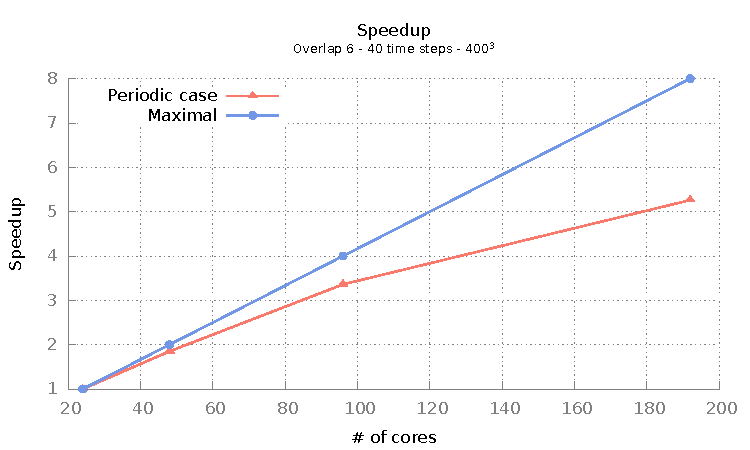
\includegraphics[page=1,scale=0.8]{gnuplot/bench_strong_nemo.pdf}}
    \only<2>{\includegraphics[page=2,scale=0.8]{gnuplot/bench_strong_nemo.pdf}}
    
\end{frame}


\subsection{Scalabilité faible}
\begin{frame}
  
\end{frame}

%
% Conclusion
%
\section{Conclusion}
\begin{frame}
  \begin{itemize}
  \item Version tridimensionnelle de \textit{NTMIX}
  \item Version parallèle
  \item Amériolations encore possibles
  \end{itemize}

\end{frame}


\end{document}



